\documentclass{article}
\usepackage[paperwidth=17.8cm,paperheight=6.8cm,margin=0.15cm]{geometry}
\usepackage{tikz}
\pagestyle{empty}
\pdfinfo{/Author (RISC-V CPU) /Creator () /Producer ()}
\begin{document}\noindent
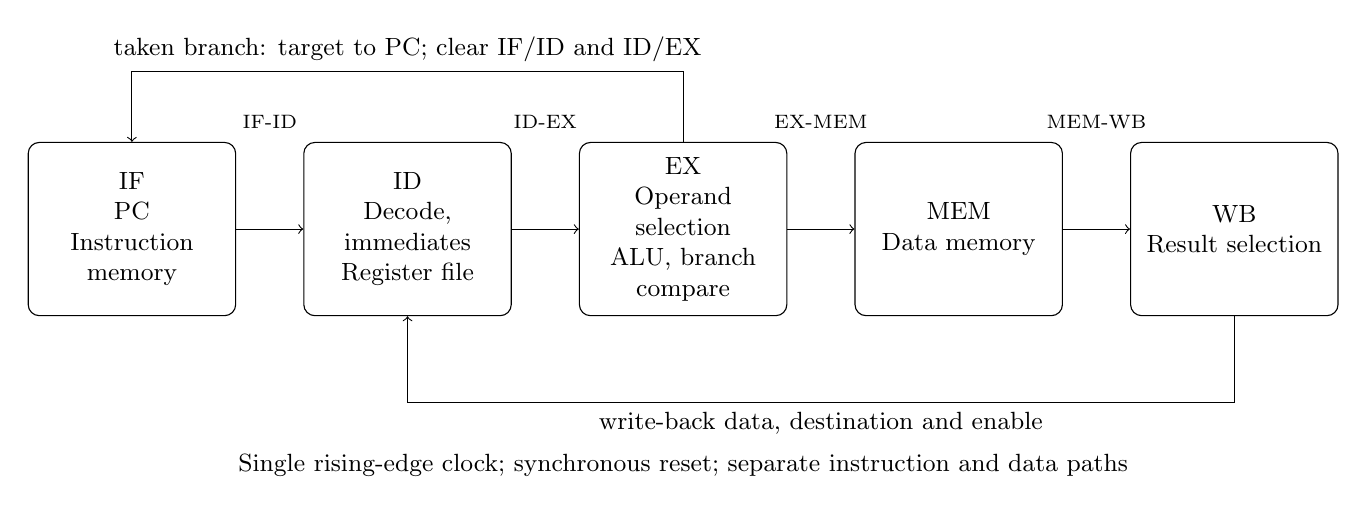
\begin{tikzpicture}[x=1cm,y=1cm, every node/.style={font=\small,align=center}, box/.style={draw,rounded corners,text width=2.4cm,minimum height=2.2cm}]
\node[box] (f) at (1.5,3) {IF\\PC\\Instruction memory};
\node[box] (d) at (5,3) {ID\\Decode, immediates\\Register file};
\node[box] (e) at (8.5,3) {EX\\Operand selection\\ALU, branch compare};
\node[box] (m) at (12,3) {MEM\\Data memory};
\node[box] (w) at (15.5,3) {WB\\Result selection};
\foreach \a/\b/\lab in {f/d/IF-ID,d/e/ID-EX,e/m/EX-MEM,m/w/MEM-WB} {
 \draw[->] (\a) -- node[above,yshift=1.15cm,font=\scriptsize]{\lab} (\b);
}
\draw[->] (w.south) -- (15.5,0.8) -- node[below]{write-back data, destination and enable} (5,0.8) -- (d.south);
\draw[->] (e.north) -- (8.5,5) -- node[above]{taken branch: target to PC; clear IF/ID and ID/EX} (1.5,5) -- (f.north);
\node at (8.5,0) {Single rising-edge clock; synchronous reset; separate instruction and data paths};
\end{tikzpicture}\end{document}
